\section{Описание эксперимента}
Эксперимент работы конвейера проводится на строчках длиной 2 миллиона символов, всего обработано 50 задач. В качестве результата приведены данные о времени начала и завершения обработки конвейерами для каждой задачи. Также вычисляются и демонстрируются минимально, максимальное и среднее время обработки задачи и простоя в очереди.

\section{Результат эксперимента}
Результаты эксперимента представлены на рисунке 4.1. Время указано в милисекундах.

\begin{figure}[h]
	\begin{center}
		{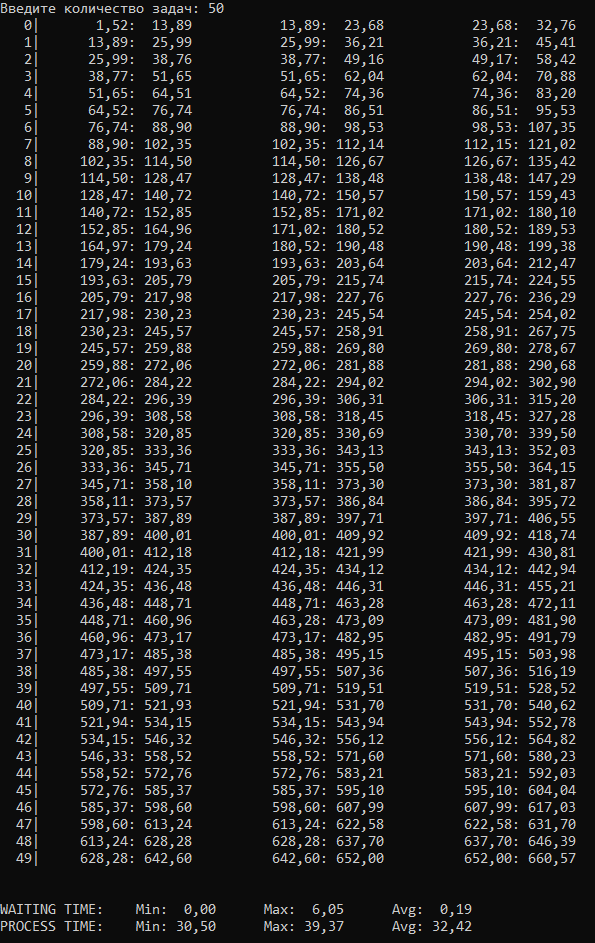
\includegraphics[scale = 1.2]{log}}
		\caption{Результаты эксперимента}
	\end{center}
\end{figure}

\section{Характеристики ПК}
Эксперименты проводились на компьютере с характеристиками:
\begin{itemize}
	\item ОС - Windows 10, 64 бит;
	\item Процессор -  Intel Core i7 8550U (1800 МГц, 4 ядра, 8 логических процессоров);
	\item Объем ОЗУ: 8 ГБ.
\end{itemize}

% //////////////
\section*{Вывод}
По результатам экспериментов можно заключить следующее.
\begin{itemize}
	\item Среднее время обработки задачи примерно в 160 раз больше времени ожидания задачи в очереди и диспетчеризации.
	\item Максимальное время простоя в очереди приблезительно в 5 раз меньше среднего времени обработки задчи. 
	\item Оба предыдущих вывода показывают, что время диспетчеризации и простоя в любом случае значительно меньше, чем время активной обработки задачи лентами конвейера.
	\item Минимальное и максимальное время обработки имеют различие лишь на 30\%.
	\item Ввиду пренебрежимости времени диспетчеризации, можно утверждать, что минимальное время обработки задачи равно времени, которое было бы затрачено в случае использования неконвейерного алгоритма. Тогда в среднем каждая задача в конвейерном алгоритме обрабатывается лишь на $6\%$ дольше, чем в алгоритме без конвейера.
	\item На обработку всех 50 задач было затрачено примерно 660 мс. Из пункта выше можно предположить, что алгоритм без конвейера затратил был $30.5*50 = 1525$ мс, что в 2.3 раза дольше, чем в изученной реализации.
\end{itemize}


	